\section{Methodology}
To better express the discontinuity of the 3D surface, based on AtlasNet, we sample the points from 2D patch based on learned importance map instead of uniform distribution. Our method is visualized in Figure~\ref{fig:overview}.

\begin{figure}[t]
	\begin{center}
		\includegraphics[width=0.8\linewidth]{img/overview}
	\end{center}
	\caption{Overview}
	\label{fig:overview}
\end{figure}

\subsection{Importance Loss}
To learn the importance map, we use cross entropy loss.
\begin{equation}
-\sum P(\mathbf{z}) \ln \hat{P}(\mathbf{z})
\end{equation}
For a point from a regular grid on $[0,1]^2$, $\hat{P}(\mathbf{z})$ is calculated by bilinear interpolation from the output importance map.

\begin{equation}
P(\mathbf{z}) = \exp\{-\frac{|| f(\mathbf{z}) - \min_{y}||f(\mathbf{z}) - y||^2 ||^2}{\sigma^2}  \},
\end{equation}

$\mathbf{x}=f(\mathbf{z})$ is the learned MLP that map from the predefined patch to output 3D points $\mathbf{x}$.
$min_y(||f(\mathbf{z}) - y|| )$ means find the nearest point of $f(\mathbf{z}) $ in ground truth $Y$. $\sigma$ is chosen as one-third of average distance between any point of $Y$ and its nearest neighbor inside $Y$.

\subsection{Sampling}
\begin{algorithm}[htb] 
	\caption{ Reject Sampling } 
	\label{alg:Framwork} 
	\begin{algorithmic}[1] 
		\Require
		The target probability $p(\mathbf{z}) = \frac{\hat{P}(\mathbf{z})}{\sum \hat{P}(\mathbf{z})}$;
		Sampling Number $N$;
		\Ensure 
		N sampled 2d points ; 
		\State Sample $\mathbf{z}^* \sim q(\mathbf{z})$, $q(\mathbf{z}) = \mathcal{N}(0.5,0.5) \times \mathcal{N}(0.5,0.5)$
		\State Calculate $k = \max p(\mathbf{z}) / q(\mathbf{z})$
		\State Sample $u \sim U(0,kq(\mathbf{z^*}))$ 
		\State Accept $\mathbf{z}^*$, if $u < p(\mathbf{z^*}) $
		\State Repeat Until $N$ samples are accepted\\
		\Return The N samples; 
	\end{algorithmic} 
\end{algorithm}

\begin{figure}[t]
	\begin{center}
		\includegraphics[width=0.9\linewidth]{img/p_2190}
	\end{center}
	\caption{Sampling Result}
	\label{fig:sample}
\end{figure}



